%SI 2014-09-05

\documentclass{article}

\usepackage[T1]{fontenc}
\usepackage[utf8]{inputenc}
\usepackage[swedish]{babel}
\usepackage{fullpage}
\usepackage{amssymb}
\usepackage{bussproofs}
\usepackage{amsmath}
\usepackage{graphicx}
\usepackage{verbatim}
\usepackage{tikz}
\let\emptyset\varnothing


\title{Supplemental Instructions}
\author{Erik Thorsell \\ 
		\small{erithor@student.chalmers.se}
}
\date{2015-10-15}

\begin{document}
\maketitle


\section*{Repetition}
Repetition är moder till all inlärning.

\subsection*{Mängder}
Låt $A$, $B$ och $C$ vara mängder. Bevisa - eller ge ett motexempel - till 
följande påståenden.
\begin{itemize}
\item[a)] $A \cap (B \backslash C) = (A \cap B) \backslash (A \cap C)$
\item[b)] $A \cup (B \backslash C) = (A \cup B) \backslash (A \cup C)$
\item[c)] $A \backslash B = B \backslash A$
\end{itemize}
{\it Tentamen 2004-01-16}

\subsection*{Induktionsbevis}
Visa att det för alla positiva heltal $n$ gäller att 
$$\sum_{k=1}^{n} \frac{k^2}{2^k} = 6 - \frac{n^2+4n+6}{2^n}$$
{\it Tentamen 2006-04-22}


\subsection*{Diofantiska ekvationer}
\begin{itemize}
\item[1.] 
Du får två hinkar. Den ena hinken rymmer 28 liter, den andra rymmer 19 liter.
Hur gör du för att med hjälp av dessa två mäta upp exakt 7 liter vatten?\\
\\
{\it Tentamen 2006-01-10}

\item[2.]
Lös den diofantiska ekvationen $$45x+50y=25$$
{\it Tentamen 2005-08-16}
\end{itemize}

\subsection*{Permutationer}
På hur många sätt kan man fördela 13 apelsiner och 10 äpplen bland 6 barn 
om varje barn ska få minst en apelsin och minst ett äpple?\\
\\
{\it Tentamen 2006-01-10}

\subsection*{Kongruens}
I en urna finns drygt 3000 kulor. Om man delar upp dessa i högar om 106 kulor 
får man 18 kulor över. Om man å andra sidan delar upp dem i högar om 94 kulor 
får man 2 kulor över. Hur många kulor är det i urnan?\\
\\
{\it Tentamen 2005-12-16}


\section*{Grafer}

\begin{comment}
In graph theory, an isomorphism of graphs $G$ and $H$ is a bijection between 
the vertex sets of $G$ and $H$ $$f \colon V(G) \rightarrow V(H)$$ 
such that any two vertices $u$ and $v$ of $G$ are adjacent in $G$ if and only 
if $f(u)$ and $f(v)$ are adjacent in $H$. This kind of bijection is generally 
called ``edge-preserving bijection'', in accordance with the general notion of 
isomorphism being a structure-preserving bijection.\\
\\
If an isomorphism exists between two graphs, then the graphs are called 
isomorphic and we write $G \simeq H$. In the case when the bijection is a 
mapping of a graph onto itself, i.e., when $G$ and $H$ are one and the same 
graph, the bijection is called an automorphism of $G$.\\
\\
The graph isomorphism is an equivalence relation on graphs and as such it 
partitions the class of all graphs into equivalence classes. A set of graphs 
isomorphic to each other is called an isomorphism class of graphs.\\
\\
The two graphs shown below are isomorphic, despite their different looking 
drawings.

Exempel på två isomorfa grafer.\\
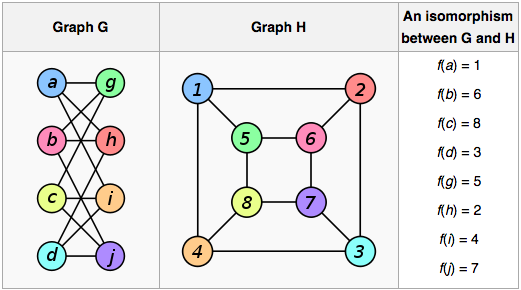
\includegraphics[scale=0.9]{isomorph.png}
\end{comment}

\begin{enumerate}

\item[1.]
Rita följande grafer:
\begin{itemize}

\item[a)]
$G = ( \{ a,b,c \} , \{ \{ a,b \} , \{ b,c \} \} )$

\item[b)]
$C_{4}$

\item[c)]
$K_{4}$

\item[d)]
$K_{5,2}$

\item[e)]
$K_{3,1}$

\item[f)]
$P_{5}$

\end{itemize}
{\it }

\item[2.]
\begin{itemize}

\item[a)]
Rita en graf med 6 noder där alla noder har gradtal 4. Finns det en Eulercykel i 
denna graf? Ange i sådana fall denna genom att sätta namn på noderna och ange i 
vilken ordning de passeras.

\item[b)]
Varför är det omöjligt att rita en graf med 7 noder där alla noder har gradtal 3?
\end{itemize}
{\it Tentamen 2005-01-11}

\item[3.]
Nedan finner du två isomorfa grafer. Finn en isomorfi mellan dem.\\
{\it Jag la ner {\bf alldeles} för mycket tid på den här uppgiften, snälla, 
lös den!}
\usetikzlibrary{positioning}
\tikzset{main node/.style={circle,fill=white,draw,minimum size=1cm, inner 
         sep=0pt},
            }

\begin{tikzpicture}
    \node[main node] (5) {$5$};
    \node[main node] (1) [below left =1cm and 1.5cm of 5]{$1$};
    \node[main node] (2) [below right=1cm and 1.5cm of 5]{$2$};
    \node[main node] (3) [below      =2.0cm         of 1]{$3$};
    \node[main node] (4) [below      =2.0cm         of 2]{$4$};

    \path[draw,thick]
    (5) edge node {} (1)
    (5) edge node {} (2)
    (1) edge node {} (2)
    (1) edge node {} (3)
    (2) edge node {} (4)
    (3) edge node {} (4);

    \begin{scope}[xshift=5cm,yshift=-3cm]
        \node[main node] (1) {$a$};
        \node[main node] (2) [right = 1cm of 1]{$b$};
        \node[main node] (3) [right = 1cm of 2]{$c$};
        \node[main node] (4) [right = 1cm of 3]{$d$};
        \node[main node] (5) [right = 1cm of 4]{$e$};

        \path[draw,thick]
         (1) edge node {} (2)
         (2) edge node {} (3)
         (3) edge node {} (4)
         (4) edge node {} (5)
         (1) edge [bend left] node {} (5)
         (2) edge [bend right] node {} (5);
   
    \end{scope}

\end{tikzpicture}

\subsection*{Inducerade grafer}
$G'$ är en inducerad delgraf av $G$ om alla kanter i $G$ som går mellan två noder 
som finns med i $G'$ också finns med i $G'$. De enda kanterna som tagits bort 
är alltså sådana som går till en nod som tagits bort.\\
{\it Kika på sid. 189-190 i kursboken.}

\end{enumerate}
\end{document}
